%%%%%%%%%%%%%%%%%%%%%%%%%%%%%%%%%%%%%%%%%
% Structured General Purpose Assignment
% LaTeX Template
%
% Template Name: Anthony
% The template was named after my friend Anthony.
% Strong inspired by Apache Hadoop and Java (programming language)
%
% Author: Ang LEE
%
% Blog: http://angli.me/
%
% Github: https://github.com/leeang/
%
%%%%%%%%%%%%%%%%%%%%%%%%%%%%%%%%%%%%%%%%%

%----------------------------------------------------------------------------------------
%	CONSTANTS
%----------------------------------------------------------------------------------------

\newcommand{\hmwkTitle}{Report\ \#1}					% Assignment title
\newcommand{\hmwkClass}{Signal Processing}				% Course name
\newcommand{\hmwkClassTime}{}							% Workshop time
\newcommand{\hmwkClassInstructor}{}						% Tutor name
\newcommand{\hmwkAuthorName}{Ang LEE}					% Student name

\newcommand{\hmwkGraphicsPath}{img/}					% Graphics path
\newcommand{\hmwkCodePath}{code/}						% Code path

%----------------------------------------------------------------------------------------
%	TEMPLATE
%----------------------------------------------------------------------------------------

\documentclass{article}

\usepackage{fancyhdr}	% Required for custom headers
\usepackage{lastpage}	% Required to determine the last page for the footer
\usepackage{extramarks} % Required for headers and footers
\usepackage{graphicx}	% Required to insert images
\graphicspath{\hmwkGraphicsPath}
\usepackage{lipsum} 	% Used for inserting dummy 'Lorem ipsum' text into the template

\usepackage{float}
\usepackage{epstopdf}	% Required to insert .eps images
\usepackage{amssymb}
\usepackage{amsmath}
\usepackage[hidelinks]{hyperref}

% MATLAB syntax highlighting
\usepackage{color}		% Required to define colors
\definecolor{commentColor}{RGB}{34,139,34}
\definecolor{stringColor}{RGB}{160,32,240}
\usepackage{listings}
\lstset{
	inputpath=\hmwkCodePath,
	language=Matlab,
	basicstyle=\footnotesize\ttfamily,
	keywordstyle=\color{blue},
	stringstyle=\color{stringColor},
	commentstyle=\usefont{T1}{pcr}{m}{n}\color{commentColor},
	breaklines=true,
	showstringspaces=false
}

% Margins
\topmargin=-0.45in
\evensidemargin=0in
\oddsidemargin=0in
\textwidth=6.5in
\textheight=9.0in
\headsep=0.25in

\linespread{1.1}		% Line spacing

% Set up the header and footer
\pagestyle{fancy}
\lhead{\hmwkTitle} % Header Left 
\chead{\hmwkAuthorName} % Header Center
\rhead{\hmwkClass} % Header Right
\lfoot{\url{https://github.com/leeang/Signal-Processing}} % Footer Left
\cfoot{} % Footer Center
\rfoot{Page\ \thepage\ of\ \pageref{LastPage}} % Footer Right
\renewcommand\headrulewidth{0.4pt} % Size of the header rule
\renewcommand\footrulewidth{0.4pt} % Size of the footer rule

\setlength\parindent{0pt} % Removes all indentation from paragraphs

%----------------------------------------------------------------------------------------
%	Problem and Section
%----------------------------------------------------------------------------------------

\newenvironment{homeworkProblem}[1]{
	\section*{#1}
	}{
}
\newenvironment{homeworkSection}[1]{
	\subsection*{#1}
	}{
}
\newcommand{\problemAnswer}[1]{
	\noindent\framebox[\columnwidth][c]{
		\begin{minipage}{0.98\columnwidth}
			#1
		\end{minipage}
	}
}
\newcommand\definiteInt[1]{		% definite integral
	\left.{#1}\vphantom{\Big|}\right|
}

%----------------------------------------------------------------------------------------
%	Document
%----------------------------------------------------------------------------------------

\begin{document}

\newpage

%----------------------------------------------------------------------------------------
%	PROBLEM 1
%----------------------------------------------------------------------------------------

% To have just one problem per page, simply put a \clearpage after each problem

\begin{homeworkProblem}{A Questions}

\begin{homeworkSection}{a)}

Given a continuous time signal 


\begin{equation}\label{Aa1}
x_c(t)=
\begin{cases} e^{-at}\cos{(\Omega_1t)} & \quad t\geq0,a>0\\ 0 & \quad t<0\\ \end{cases}
\end{equation}

Driven an expression for the spectrum $X_c(j\Omega)$. Plot $x_c(t)$ and $X_c(j\Omega)$ in Matlab.


\begin{figure}[H]
\begin{minipage}[t]{0.5\linewidth}
\centering
\includegraphics[width=3.3in]{Q1a-time-different-a.eps}
\caption{$x_c(t)$ for various $a$}
\label{xt1}
\end{minipage}
\begin{minipage}[t]{0.5\linewidth}
\centering
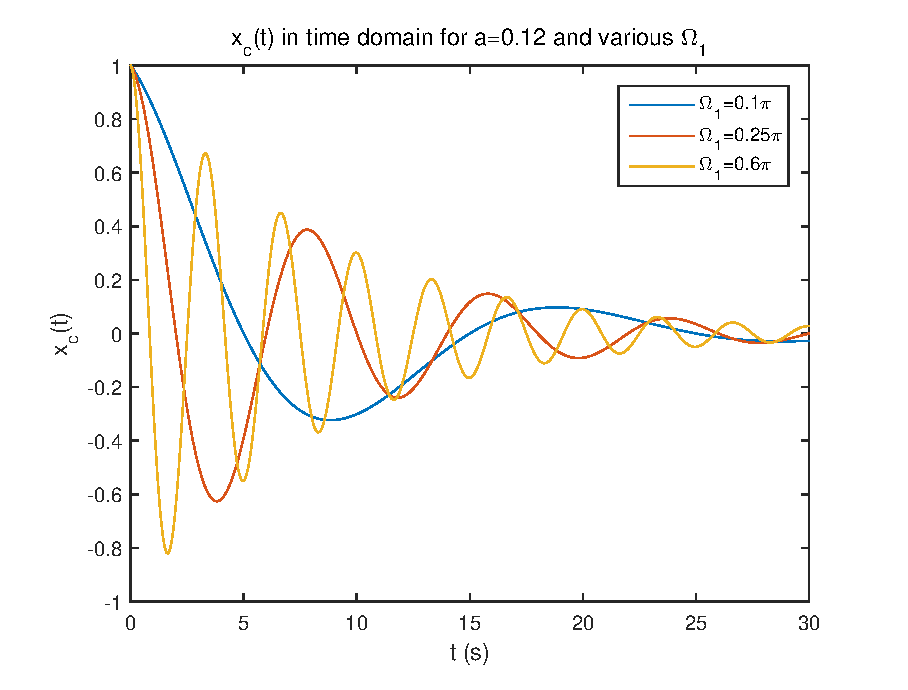
\includegraphics[width=3.3in]{Q1a-time-different-Omega.eps}
\caption{$x_c(t)$ for various $\Omega_1$}
\label{xt2}
\end{minipage}
\end{figure}


\begin{figure}[H]
\begin{minipage}[t]{0.5\linewidth}
\centering
\includegraphics[width=3.3in]{Q1a-frequency-different-a.eps}
\caption{$X_c(\Omega)$ for various $a$}
\label{fig:side:a}
\end{minipage}
\begin{minipage}[t]{0.5\linewidth}
\centering
\includegraphics[width=3.3in]{Q1a-frequency-different-Omega.eps}
\caption{$X_c(\Omega)$ for various $\Omega_1$}
\label{fig:side:b}
\end{minipage}
\end{figure}


\problemAnswer{
\vspace{10pt}
Take Fourier transform on Eq.\ref{Aa1} to get the spectrum of the original signal.

\begin{align*}
X_c(j\Omega) &=\int_0^{\infty}e^{-at}\cos{(\Omega_1t)}e^{-j\Omega t}dt \quad (\text{since the original signal only has value when } t\geq 0)\\
&= \int_{0}^{\infty}e^{-at}\frac{e^{j\Omega_1t}+e^{-j\Omega_1t}}{2}e^{-j\Omega t}dt \\
&= \frac{1}{2}\int_{0}^{\infty}e^{(-a+j\Omega_1-j\Omega)t}+e^{(-a-j\Omega_1-j\Omega)t}dt\\
&= \frac{1}{2}\definiteInt{\frac{1}{-a+j\Omega_1-j\Omega}e^{(-a+j\Omega_1-j\Omega)t}}_0^\infty+\frac{1}{2}\definiteInt{\frac{1}{-a-j\Omega_1-j\Omega}e^{(-a-j\Omega_1-j\Omega)t}}_0^\infty\\
&= \frac{1}{2}[\frac{-1}{-a+j(\Omega_1-\Omega)}+\frac{-1}{-a-j(\Omega_1+\Omega)}]\\
&=\frac{1}{2}\frac{a+j(\Omega_1+\Omega)+a-j(\Omega_1-\Omega)}{(-a+j(\Omega_1-\Omega))(-a-j(\Omega_1+\Omega))}\\
&=\frac{a+j\Omega}{a^2+2aj\Omega+\Omega_1^2-\Omega^2}\\
&=\frac{a+j\Omega}{(a+j\Omega)^2+\Omega_1^2}\\
\end{align*}

As $a$ increases, signal decays more rapidly in time domain while the magnitudes become smaller and the peaks move slightly farther away from the symmetry axis in frequency domain.\\

When $\Omega_1$ grows, signal fluctuates more sharply in time domain. In terms of frequency domain, the spectrum spread wider and the peaks move farther away from the symmetry axis. The magnitude decreases marginally.
}

\end{homeworkSection}

\begin{homeworkSection}{b)}
Let the sample version of $x_c(t)$ be $x[n]=x_c(nT)$. Calculate the DTFT $X(e^{j\omega})$ for the sampled signal.

\problemAnswer{
\vspace{10pt}
The DTFT of discrete time signal $x[n]$ is
\begin{align*}
X(e^{j\omega})&=\sum_{-\infty}^{\infty}x[n]e^{-j\omega n}\\
&= \sum_{0}^{\infty}e^{-anT}\cos{(\Omega_1nT)}e^{-j\omega n}\\
&= \sum_{0}^{\infty}e^{-anT}\frac{e^{j\Omega_1 nT}+e^{-j\Omega_1 nT}}{2}e^{-j\omega n}\\
&= \frac{1}{2}\sum_{0}^{\infty}(e^{-anT+j\Omega_1 nT-j\omega n}+e^{-anT-j\Omega_1 nT-j\omega n})\\
&= \frac{1}{2}(\frac{1}{1-e^{-aT+j(\Omega_1T-\omega)}}+\frac{1}{1-e^{-aT-j(\Omega_1T+\omega)}})\\
&= \frac{1}{2}\frac{2-e^{-aT-j(\Omega_1T+\omega)}-e^{-aT+j(\Omega_1T-\omega)}}{(1-e^{-aT+j(\Omega_1T-\omega)})(1-e^{-aT-j(\Omega_1T+\omega)})}\\
&= \frac{1-e^{-aT}\cos(\Omega_1 T)e^{-j\omega}}{1-2e^{-aT}\cos(\Omega_1 T)e^{-j\omega}+e^{-2aT}e^{-2j\omega}}\\
\end{align*}
}
\end{homeworkSection}


\begin{homeworkSection}{c)}
Let $a=0.12$ , $\Omega_1=0.25\pi$ and let the sampling frequency $F$=4.8Hz. Plot $X_c(j\Omega)$ and $X(e^{j\omega})$ in Matlab.Do necessary scalings to match them up. Explain the command freqz in Matlab.

\begin{figure}[H]
\centering
\includegraphics[scale=0.7]{Q1c.eps}
\caption{$X_c(j\Omega)$ and $X(e^{j\omega})$}
\label{Qc}
\end{figure}

\problemAnswer{
\vspace{10pt}

According to the lecture slides $1-9/23$ and $1-18/23$, the process of recovering $X_c(j\Omega)$ from $X(e^{j\omega})$ depends on sampling period $T$.

\begin{equation}
X(e^{j\omega})=\frac{1}{T}\sum_{k=-\infty}^{\infty}X_c(j(\Omega+k\Omega_T))
\end{equation}

In order to match the spectrum of continuous time signal, we will scale the magnitude of $X(e^{j\omega})$ by a factor of $T$, in this case, $T=\frac{1}{4.8}$. Since the spectrum of $X(e^{j\omega})$ has period of $2\pi$, we need to convert the discrete $\omega$ into continuous $\Omega$ by $\Omega=\frac{\omega}{T}$.\\

In terms of the mode used in this question, three arguments are passed to the freqz function.\\
1. the coefficient before $e^{-j n \omega}$ of the numerator of $X(e^{j\omega})$\\
2. the coefficient before $e^{-j n \omega}$ of the denominator of $X(e^{j\omega})$\\
3. the $\omega$ range
}

\end{homeworkSection}

\begin{homeworkSection}{d)}
A simple first order digital lowpass filter is given by 
\begin{equation}\label{Ad1}
H_{LP}(z)=\frac{1-\alpha}{2}\frac{1+z^{-1}}{1-\alpha z^{-1}}
\end{equation}
Show that 
\begin{equation}\label{Ad2}
|H_{LP}(e^{j\omega})|^2=\frac{(1-\alpha)^2(1+\cos\omega)}{2(1+\alpha^2-2\alpha\cos\omega)}
\end{equation}
For which values of $\alpha$ is the filter stable? Plot $|H_{LP}(e^{j\omega})|$ and $\angle H_{LP}(e^{j\omega})$ for some values of $\alpha$. Comment on the results.\\

\problemAnswer{
\vspace{10pt}
Substitute $z=e^{j\omega}$ into Eq.\ref{Ad2}, yields

\begin{align*}
|H_{LP}(e^{j\omega})|^2&=\left|\frac{1-\alpha}{2}\frac{1+e^{-j\omega}}{1-\alpha e^{-j\omega}}\right|^2\\
&= \frac{(1-\alpha)^2}{4}\left|\frac{1+\cos\omega-j\sin\omega}{1-\alpha(\cos\omega-j\sin\omega)}\right|^2\\
&= \frac{(1-\alpha)^2}{4}\frac{(1+\cos\omega)^2+(-\sin\omega)^2}{(1-\alpha\cos\omega)^2+(-\alpha\sin\omega)^2}\\
&=  \frac{(1-\alpha)^2}{4}\frac{2+2\cos\omega}{1-2\alpha\cos\omega+\alpha^2}\\
&= \frac{(1-\alpha)^2(1+\cos\omega)}{2(1+\alpha^2-2\alpha\cos\omega)}\\
\end{align*}
}

\begin{figure}[H]
\begin{minipage}[t]{0.5\linewidth}
\centering
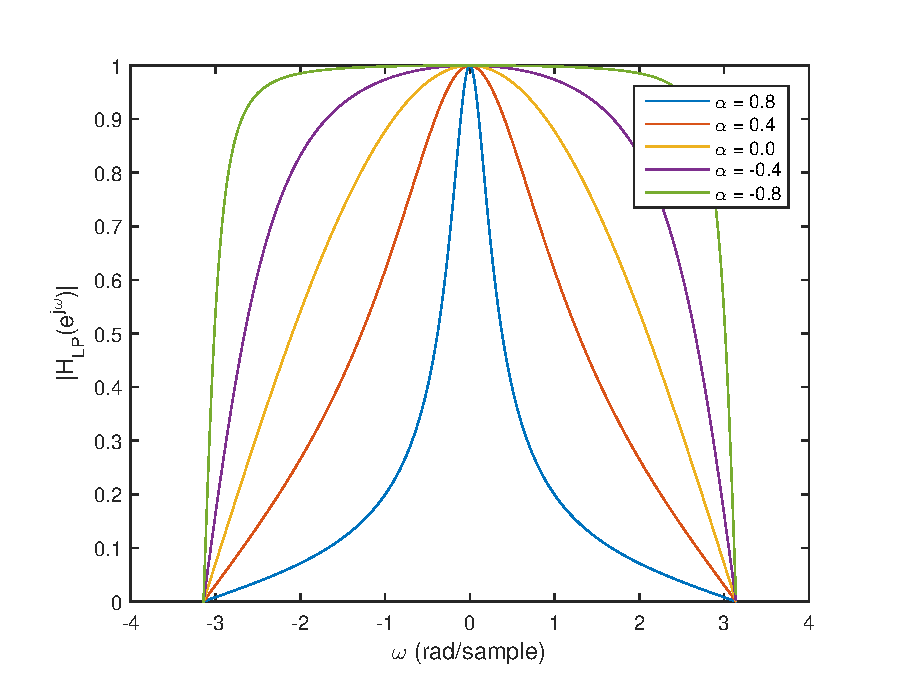
\includegraphics[width=3.3in]{Q1d-magnitude.eps}
\caption{Plot of $|H_{LP}(e^{j\omega})|$}
\label{Q1d-magnitude}
\end{minipage}
\begin{minipage}[t]{0.5\linewidth}
\centering
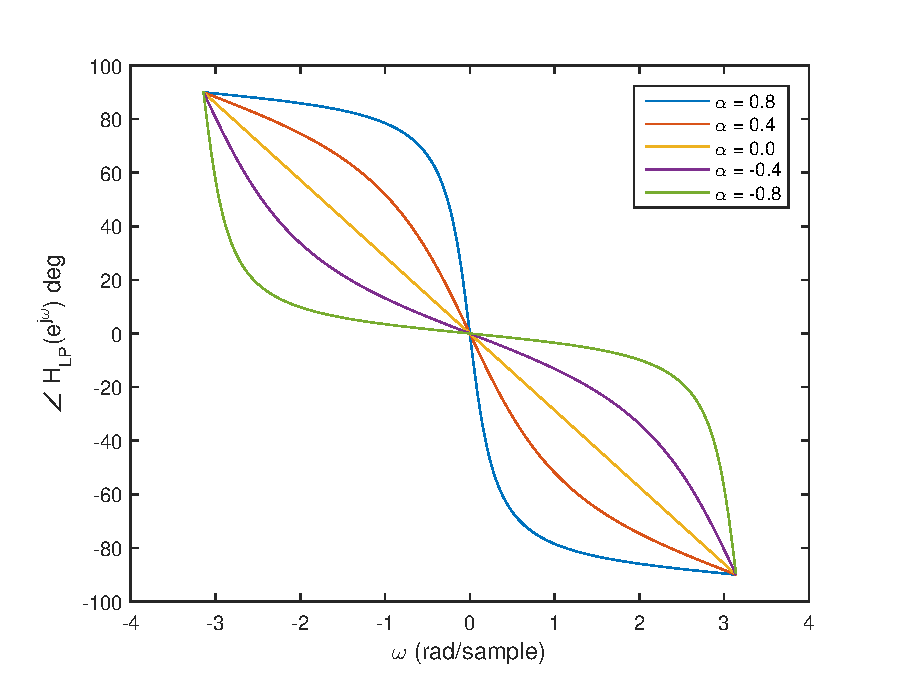
\includegraphics[width=3.3in]{Q1d-phase.eps}
\caption{Plot of $\angle H_{LP}(e^{j\omega})$}
\label{Q1d-phase}
\end{minipage}
\end{figure}

\problemAnswer{
\vspace{10pt}
The pole of the filter $z=\alpha$ should be strictly inside the unit circle, i.e.
\begin{equation}
|\alpha| < 1
\end{equation}

For simplicity, only positive $\omega$ will be discussed, because frequency domain plots are symmetric about $\omega = 0$.\\

For bigger $\alpha$, e.g. 0.8 comparing with 0.4 or - 0.8, the magnitude decreases more quickly at lower frequencies and more slowly at higher frequencies. However, for smaller $\alpha$, the magnitude decreases more slowly at lower frequencies and decreases more quickly at higher frequencies. When $\alpha$ increases, the low-pass filter becomes more capable to reject high frequency components.\\

For bigger $\alpha$, the phase decreases more slowly at lower frequencies and more quickly at higher frequencies. However, for smaller $\alpha$, the phase decreases more quickly at lower frequencies and decreases more slowly at higher frequencies. However, for larger $\alpha$, huger phase shift is inevitable.
}
\end{homeworkSection}

\end{homeworkProblem}

\begin{homeworkProblem}{B Implementation of digital anti-aliasing filters on a DSP}
\begin{homeworkSection}{B.4 Lab tasks}

%--------------------------------------------

\subsubsection*{a)}

Increase the length of the signal to 256, Figure \ref{skeleton-time} and \ref{skeleton-frequency} are the signal in time domain and frequency domain. As can be seen in Figure \ref{skeleton-frequency}, the spectrum achieve a peak value at $f=0.125\text{Hz}$ which equals to $\Omega_1=0.25\pi$ in code SPWS1.c. 

\begin{figure}[H]
\centering
\includegraphics[width=6.6in]{skeleton-time}
\caption{skeleton function in time domain}
\label{skeleton-time}
\end{figure}

\begin{figure}[H]
\centering
\includegraphics[width=6.6in]{skeleton-frequency}
\caption{skeleton function in frequency domain}
\label{skeleton-frequency}
\end{figure}

%--------------------------------------------

\subsubsection*{c)}

Figure \ref{Q2c-time}, \ref{Q2c-frequency-12} and \ref{Q2c-frequency-48} are plotted by MATLAB. Figure \ref{Q2c-time-CCES}, \ref{Q2c-frequency-12-CCES} and \ref{Q2c-frequency-48-CCES} are plotted by CCES.

\begin{figure}[H]
\centering
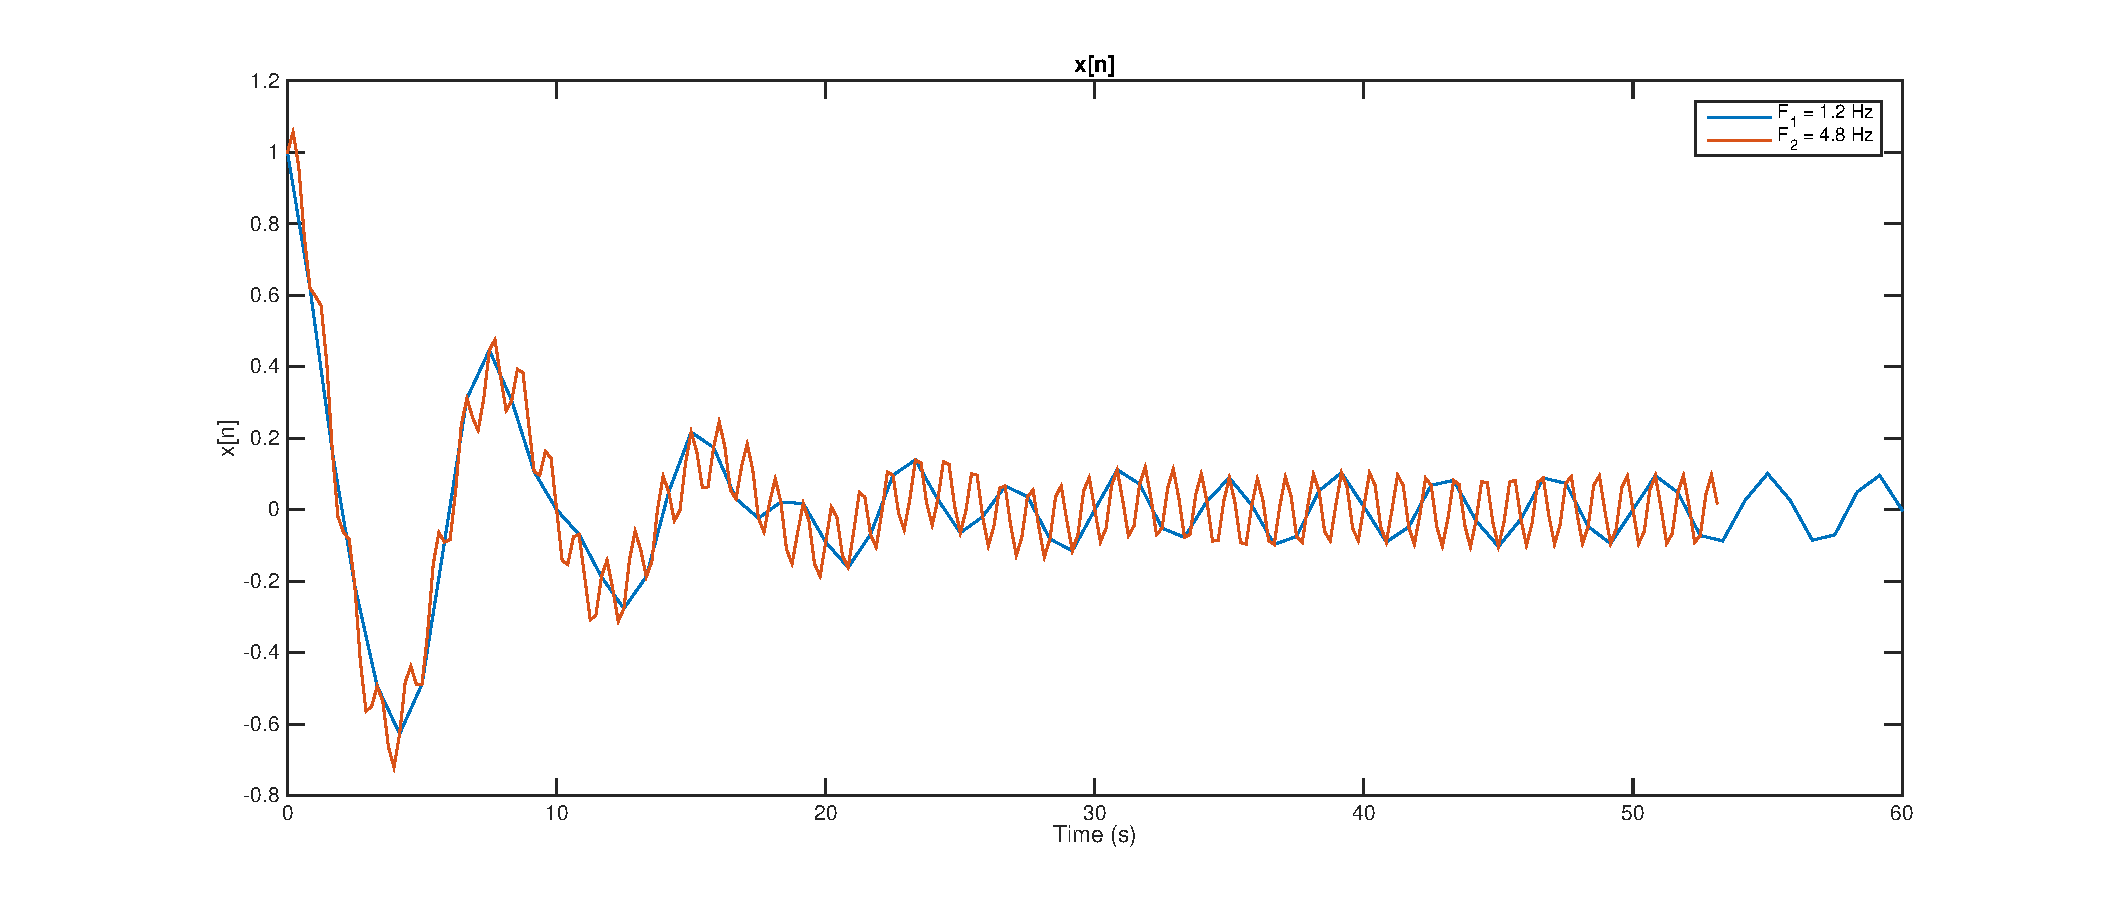
\includegraphics[width=6in]{Q2c-time.eps}
\caption{$x[n]$ in time domain (MATLAB)}
\label{Q2c-time}
\end{figure}

\begin{figure}[H]
\centering
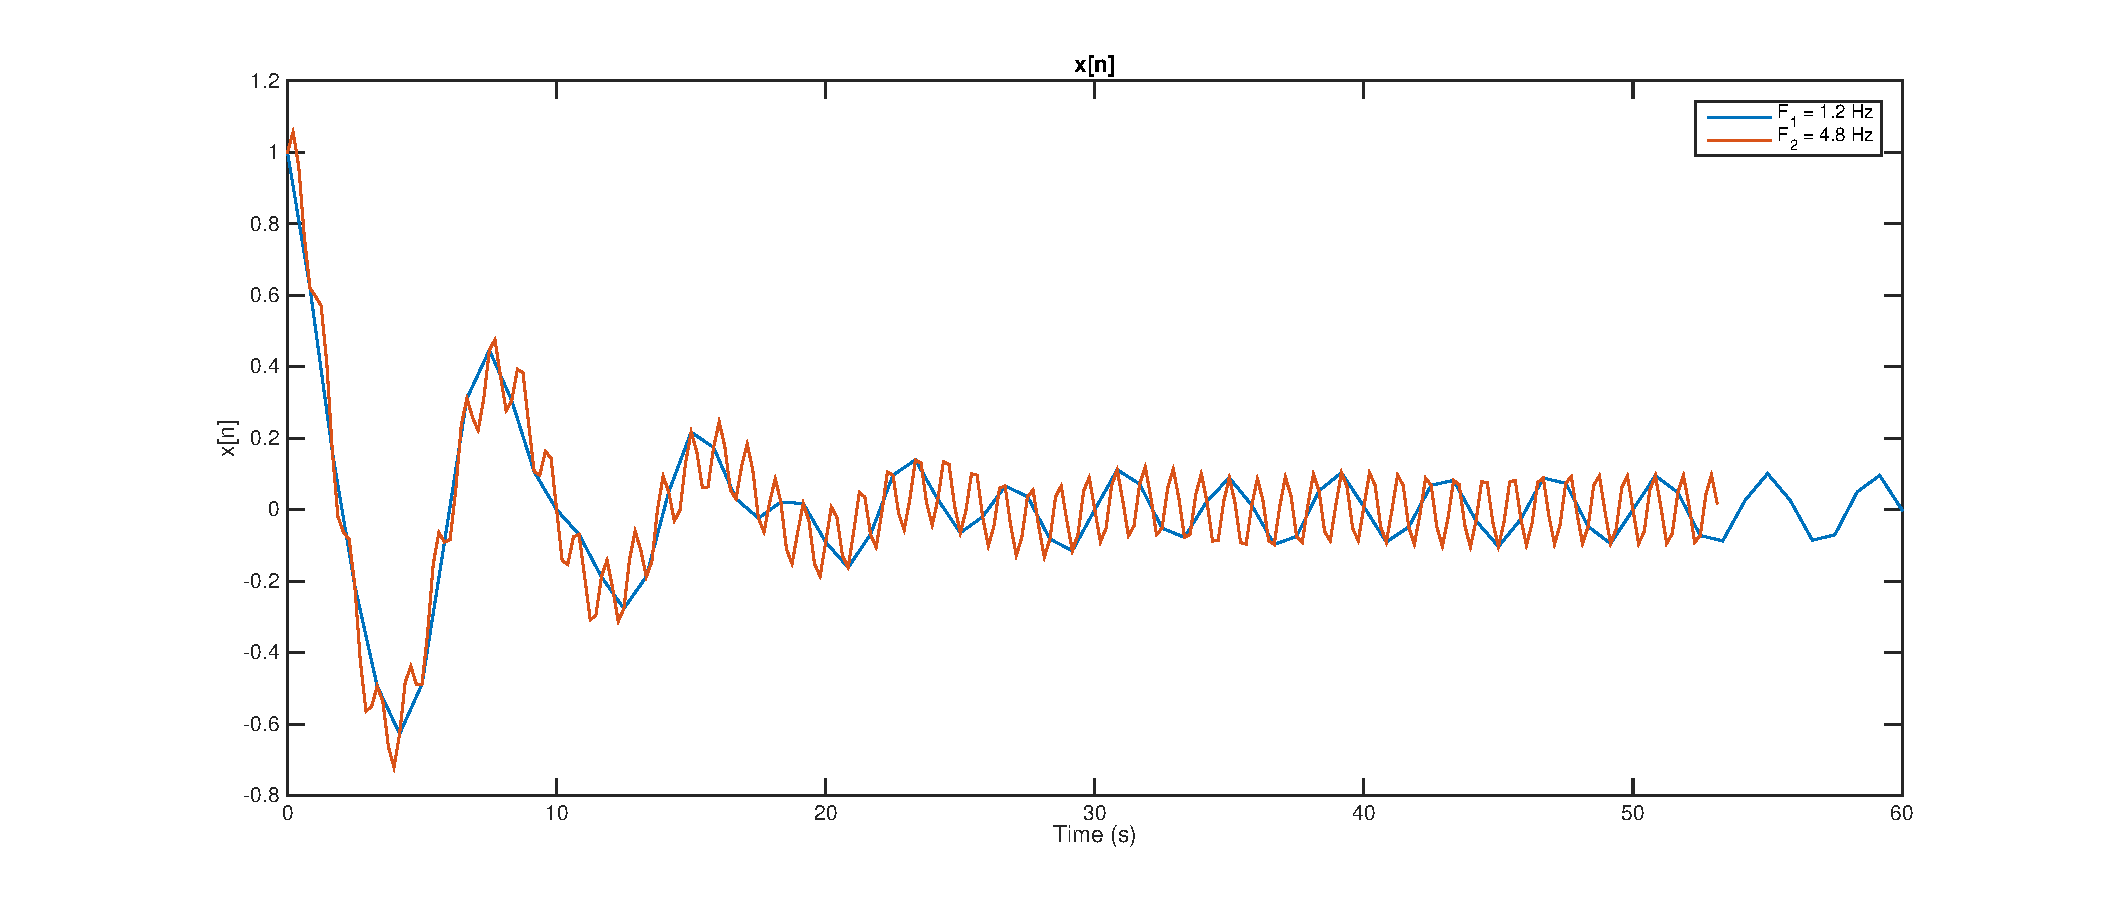
\includegraphics[width=6.6in]{Q2c-time}
\caption{$x[n]$ in time domain (CCES)}
\label{Q2c-time-CCES}
\end{figure}

\begin{figure}[H]
\begin{minipage}[t]{0.5\linewidth}
\centering
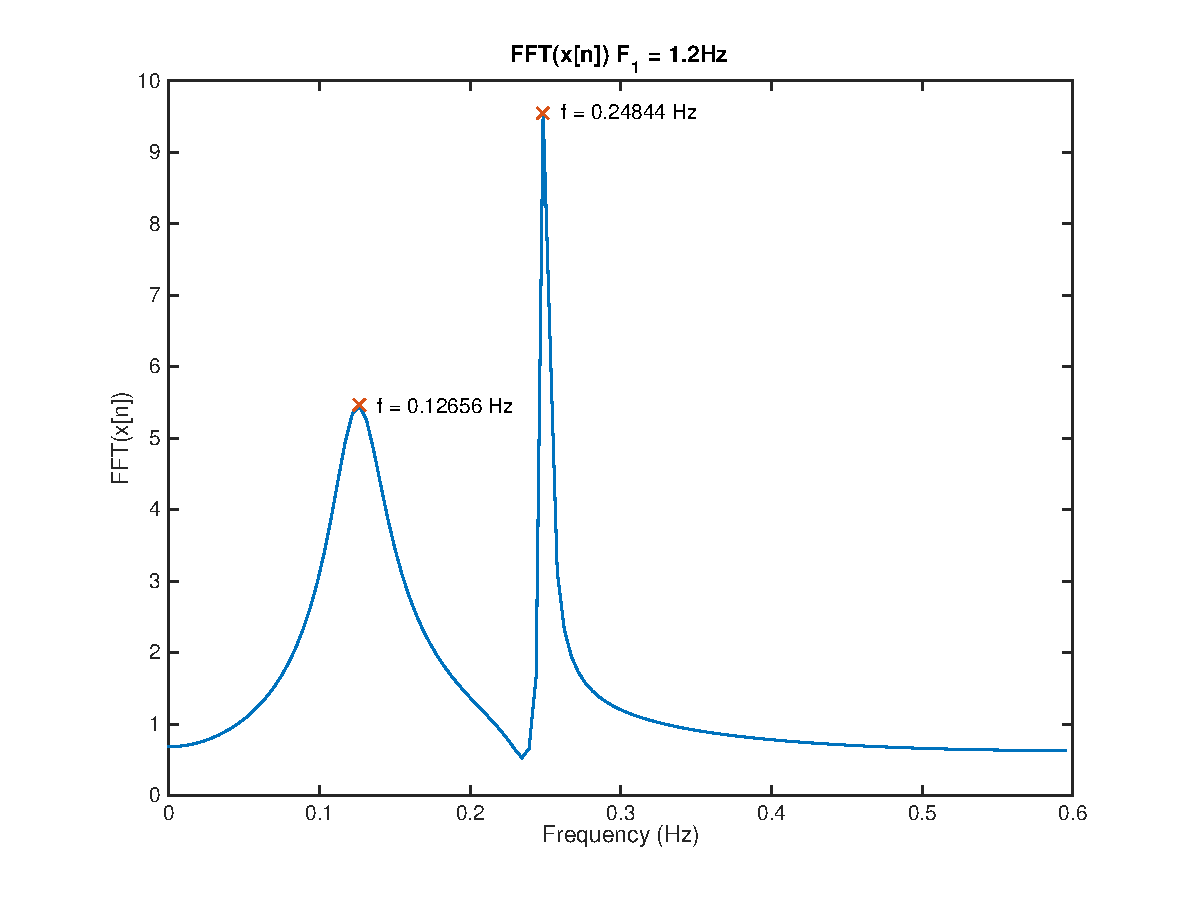
\includegraphics[width=3.3in]{Q2c-frequency-12.eps}
\caption{$x[n]$ (1.2Hz) (MATLAB)}
\label{Q2c-frequency-12}
\end{minipage}
\begin{minipage}[t]{0.5\linewidth}
\centering
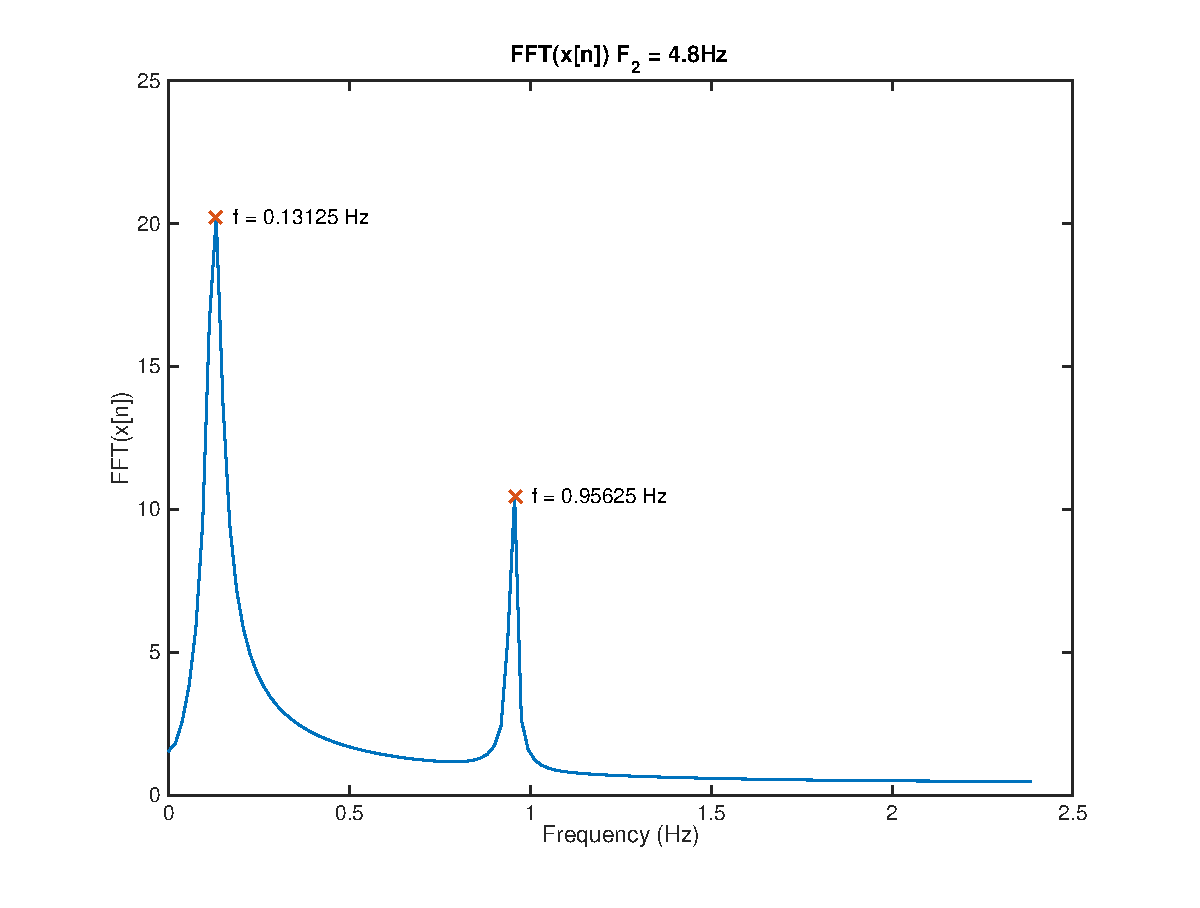
\includegraphics[width=3.3in]{Q2c-frequency-48.eps}
\caption{$x[n]$ (4.8Hz) (MATLAB)}
\label{Q2c-frequency-48}
\end{minipage}
\end{figure}

\begin{figure}[H]
\centering
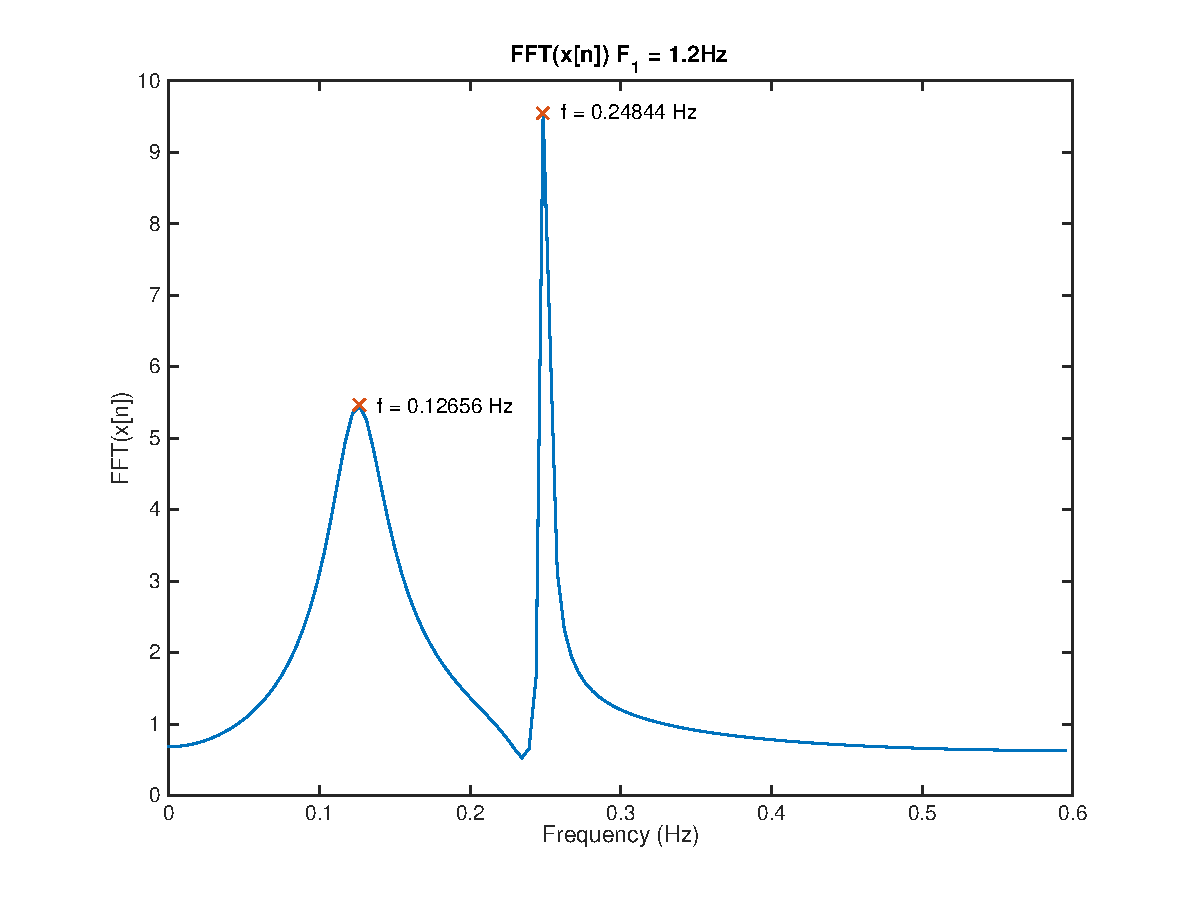
\includegraphics[width=6.6in]{Q2c-frequency-12}
\caption{$x[n]$ (1.2Hz) in frequency domain (CCES)}
\label{Q2c-frequency-12-CCES}
\end{figure}

\begin{figure}[H]
\centering
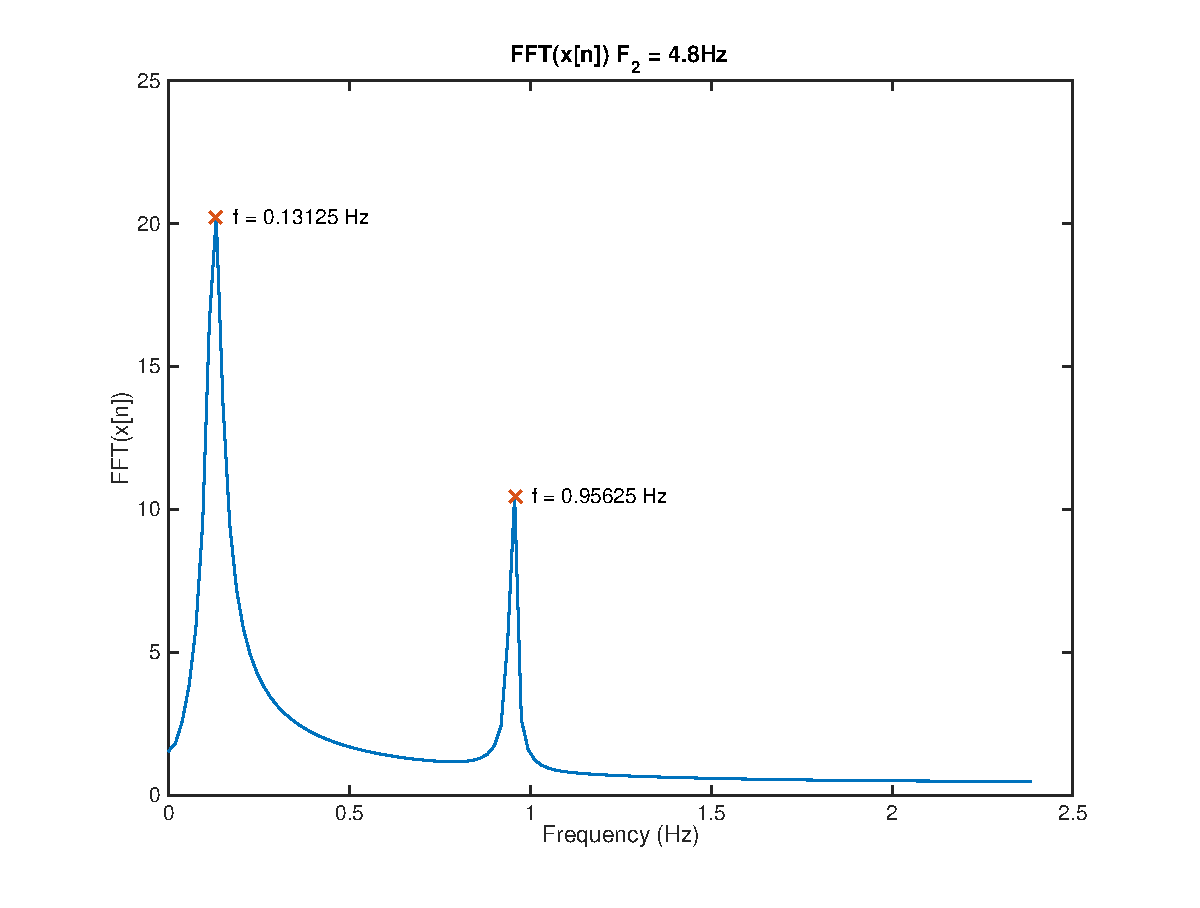
\includegraphics[width=6.6in]{Q2c-frequency-48}
\caption{$x[n]$ (4.8Hz) in frequency domain (CCES)}
\label{Q2c-frequency-48-CCES}
\end{figure}

In FFT plots, peaks near $F = \frac{\Omega_1}{2\pi} = \frac{0.25\pi}{2\pi} = 0.125$ Hz and $F = \frac{\Omega_2}{2\pi} = \frac{1.9\pi}{2\pi} = 0.95$ Hz are expected.
Figure \ref{Q2c-frequency-48} and Figure \ref{Q2c-frequency-48-CCES} (sampling frequency $F_2$ = 4.8Hz) are in agreement with this expectation.
However, an unexpected peak appears at $f \approx$ 0.24844 Hz in Figure \ref{Q2c-frequency-12} and Figure \ref{Q2c-frequency-12-CCES} (sampling frequency $F_1$ = 1.2Hz). Interestingly, we find $\frac{0.24844 + 0.95}{2}$ Hz $\approx 0.6$ Hz = $\frac{F_1}{2}$, which means this unexpected peak and the frequency of $x_2(t)$ are symmetric around $f = \frac{F_1}{2}$ (folding frequency).\\

In time domain, as is shown in Figure \ref{Q2c-time} and Figure \ref{Q2c-time-CCES}, when sampling frequency $F_2$ = 4.8Hz, higher frequency ($1.9\pi$ rad/s) fluctuation is kept; when sampling frequency $F_1$ = 1.2Hz, the oscillation frequency decreases which means higher frequency component becomes distorted.\\

In conclusion, $F_2=4.8\text{Hz}$ is a proper sampling frequency such that all the information of the original signal is obtained without aliasing and folding.

%--------------------------------------------

\subsubsection*{d)}

\begin{figure}[H]
\begin{minipage}[t]{0.5\linewidth}
\centering
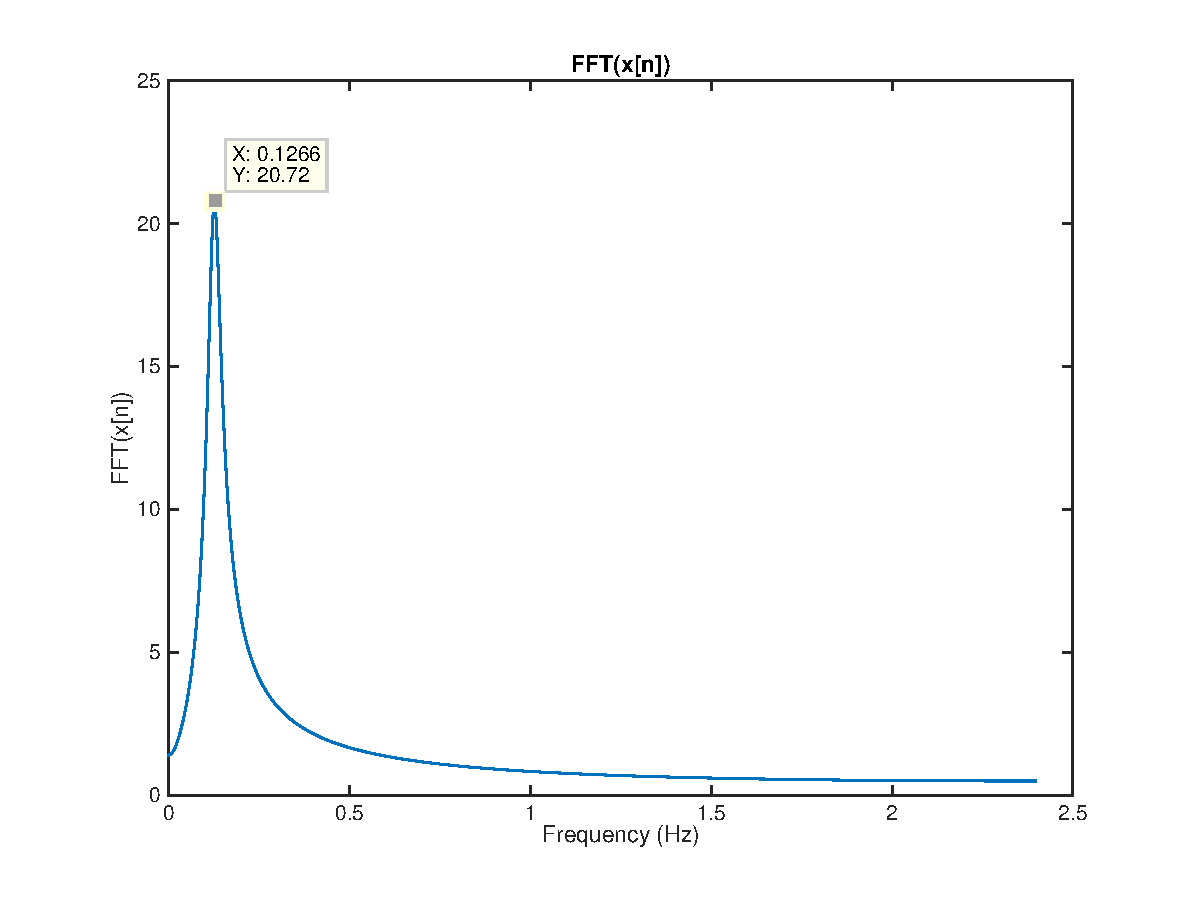
\includegraphics[width=3.3in]{Q2d_FFT.eps}
\caption{Plot of $X_1(F)$}
\label{Q2d_FFT}
\end{minipage}
\begin{minipage}[t]{0.5\linewidth}
\centering
\includegraphics[width=3.3in]{Q2d_DTFT.eps}
\caption{Plot of $X_1(e^{j\omega})$}
\label{Q2d_DTFT}
\end{minipage}
\end{figure}

As can be seen from the FFT plot (Figure \ref{Q2d_FFT}), $F_{max}$ = 0.1266 Hz, $\omega_{max} =\Omega_{max}T_{S}=\frac{0.1266}{4.8} \times 2\pi$ = 0.1657 rad/sample.\\
As is shown in the DTFT $X(e^{j\omega})$ plot (Figure \ref{Q2d_DTFT}), $\omega_{max}$ = 0.1634 rad/sample.\\

Two values of $\omega_{max}$ are consistent, we choose $\omega_{max}$ = \textbf{0.165 rad/sample}.\\

The frequency of the sinusoidal signal $x_2[n]$: $\omega_2 = \frac{1.9\pi}{4.8}$ rad/sample.\\

\textbf{(i)} a first order filter\\

From Eq.\ref{Ad2}, we obtain:
\begin{equation}\label{Bd1}
|H_{LP}(e^{j\omega})| = \frac{|1-\alpha|}{\sqrt{2}} \frac{\sqrt{1+\cos\omega}}{\sqrt{1+\alpha^2-2\alpha\cos\omega}}
\end{equation}

According to the design specification, $|H_{LP}(e^{j\omega_{max}})| = 0.95$ at $\omega_{max}$ = 0.165 rad/sample, i.e.
\begin{equation}\label{Bd2}
|H_{LP}(e^{j\omega_{max}})| = \frac{|1-\alpha_1|}{\sqrt{2}} \frac{\sqrt{1+\cos\omega_{max}}}{\sqrt{1+\alpha_1^2-2\alpha_1\cos\omega_{max}}} = 0.95
\end{equation}

Eq.\ref{Bd2} can be solved by MATLAB (assuming $-1 < \alpha_1 < 1$): $\alpha_1$ = \textbf{0.597991}.\\

At the frequency $\omega_2$, \textbf{the 1st order filter does not satisfy the design specification}, because
\begin{equation}\label{Bd3}
|H_{LP}(e^{j\omega_2})| = \frac{|1-\alpha_1|}{\sqrt{2}} \frac{\sqrt{1+\cos\omega_2}}{\sqrt{1+\alpha_1^2-2\alpha_1\cos\omega_2}} = 0.33 > 0.25
\end{equation}


\textbf{(ii)} a second order filter\\

From Eq.\ref{Ad2}, we obtain:
\begin{equation}\label{Bd4}
|H_2(e^{j\omega})| = |H_{LP}(e^{j\omega})|^2=\frac{(1-\alpha)^2(1+\cos\omega)}{2(1+\alpha^2-2\alpha\cos\omega)}
\end{equation}

According to the design specification, $|H_2(e^{j\omega_{max}})| = 0.95$ at $\omega_{max}$ = 0.165 rad/sample, i.e.
\begin{equation}\label{Bd5}
|H_2(e^{j\omega_{max}})| = |H_{LP}(e^{j\omega_{max}})|^2=\frac{(1-\alpha_2)^2(1+\cos\omega_{max})}{2(1+\alpha_2^2-2\alpha_2\cos\omega_{max})} = 0.95
\end{equation}

Eq.\ref{Bd5} can be solved by MATLAB (assuming $-1 < \alpha_2 < 1$): $\alpha_2$ = \textbf{0.470126}.\\

At the frequency $\omega_2$, \textbf{the 2nd order filter satisfies the design specification}, because
\begin{equation}\label{Bd6}
|H_2(e^{j\omega_2})| = |H_{LP}(e^{j\omega_2})|^2=\frac{(1-\alpha_2)^2(1+\cos\omega_2)}{2(1+\alpha_2^2-2\alpha_2\cos\omega_2)} = 0.20 < 0.25
\end{equation}

\problemAnswer{
\vspace{5pt}
	\lstinputlisting{Q2d_alpha_gain.m}
}

%--------------------------------------------

\subsubsection*{e)}

\textbf{First order filter time domain representation}
\begin{align*}
Y(z) &= X(z) H_{LP}(z)\\
Y(z) &= X(z) \frac{1-\alpha}{2}\frac{1+z^{-1}}{1-\alpha z^{-1}}\\
Y(z) (1-\alpha z^{-1}) &= X(z) \frac{1-\alpha}{2} (1+z^{-1})\\
Y(z) - \alpha Y(z) z^{-1} &= \frac{1-\alpha}{2} X(z) + \frac{1-\alpha}{2} X(z) z^{-1}\\
y[n] - \alpha y[n-1] &= \frac{1-\alpha}{2} x[n] + \frac{1-\alpha}{2} x[n-1] \text{ (inverse Z transform)}\\
y[n] &= \frac{1-\alpha}{2} x[n] + \frac{1-\alpha}{2} x[n-1] + \alpha y[n-1]
\end{align*}

\textbf{Second order filter time domain representation}
\begin{align*}
Y(z) &= X(z) (H_{LP}(z))^2\\
Y_1(z) &:= X(z) H_{LP}(z)\\
Y(z) &= Y_1(z) H_{LP}(z)\\
y_1[n] &= \frac{1-\alpha}{2} x[n] + \frac{1-\alpha}{2} x[n-1] + \alpha y_1[n-1] \text{ (inverse Z transform)}\\
y[n] &= \frac{1-\alpha}{2} y_1[n] + \frac{1-\alpha}{2} y_1[n-1] + \alpha y[n-1]
\end{align*}

\begin{figure}[H]
\centering
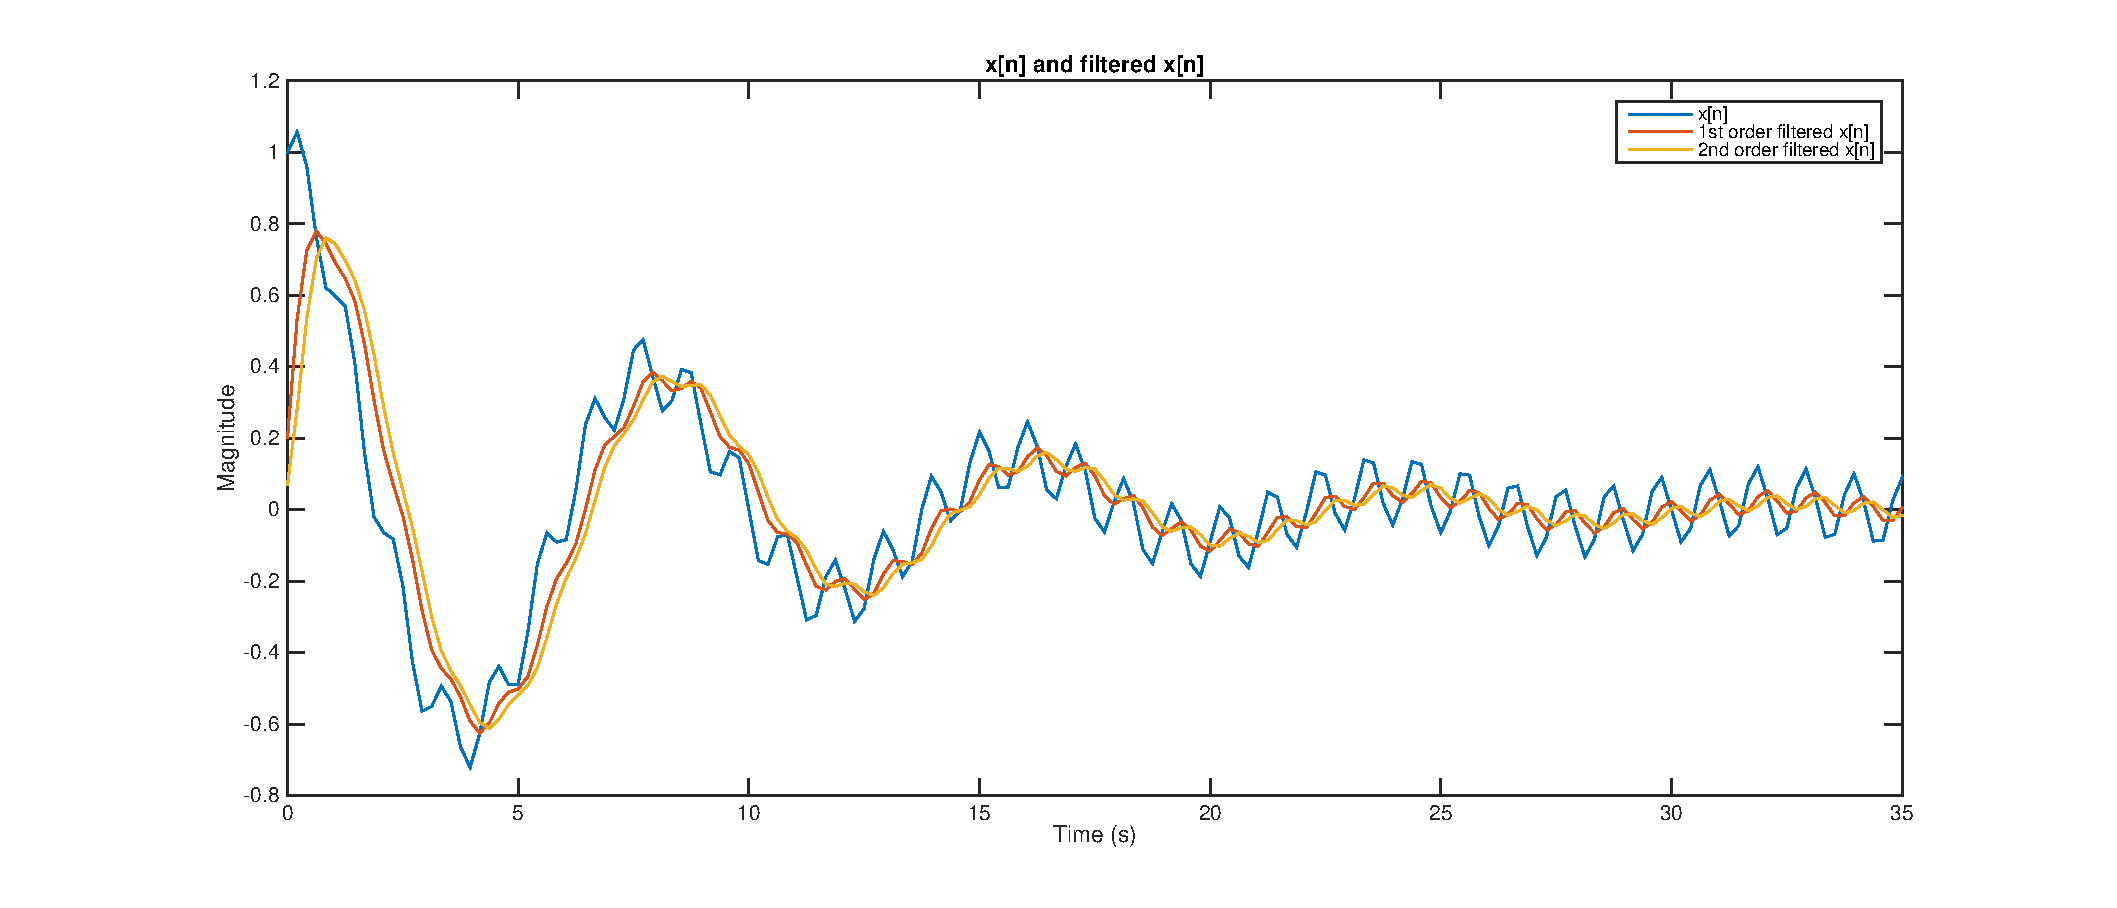
\includegraphics[width=6in]{Q2e-time.eps}
\caption{$x[n]$ and filtered $x[n]$ in time domain (MATLAB)}
\label{Q2e-time}
\end{figure}

\begin{figure}[H]
\centering
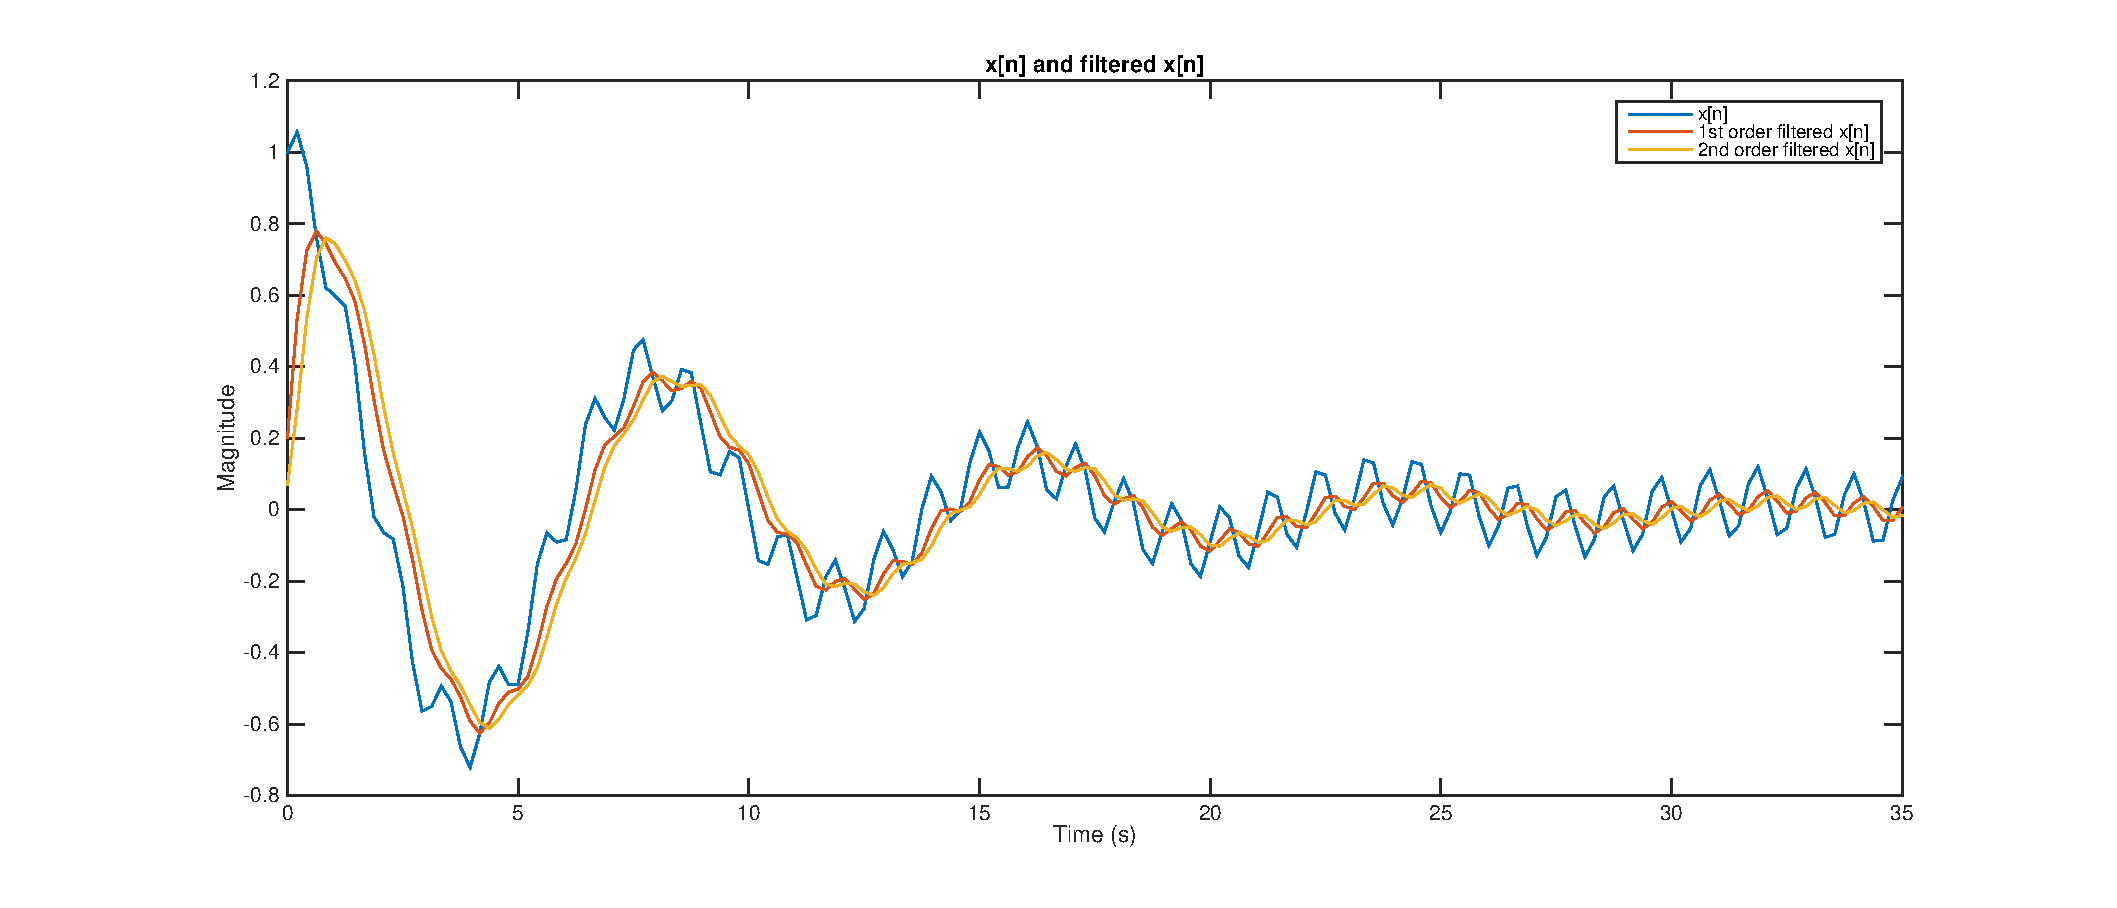
\includegraphics[width=6.6in]{Q2e-time}
\caption{$x[n]$ and filtered $x[n]$ in time domain (CCES)}
\label{Q2e-time-CCES}
\end{figure}

\problemAnswer{
\vspace{5pt}
As can bee seen from Figure \ref{Q2e-time} and Figure \ref{Q2e-time-CCES}, the magnitude of the fast oscillation period of the original signal has a peak-to-peak value 0.19 roughly. While the output signal of the first order filter is around 0.06 (larger than 25\% of 0.19). The output from the second order filter yields a 0.04 peak-to-peak value (21\% of 0.19) which satisfies the gain condition. 
}

\begin{figure}[H]
\centering
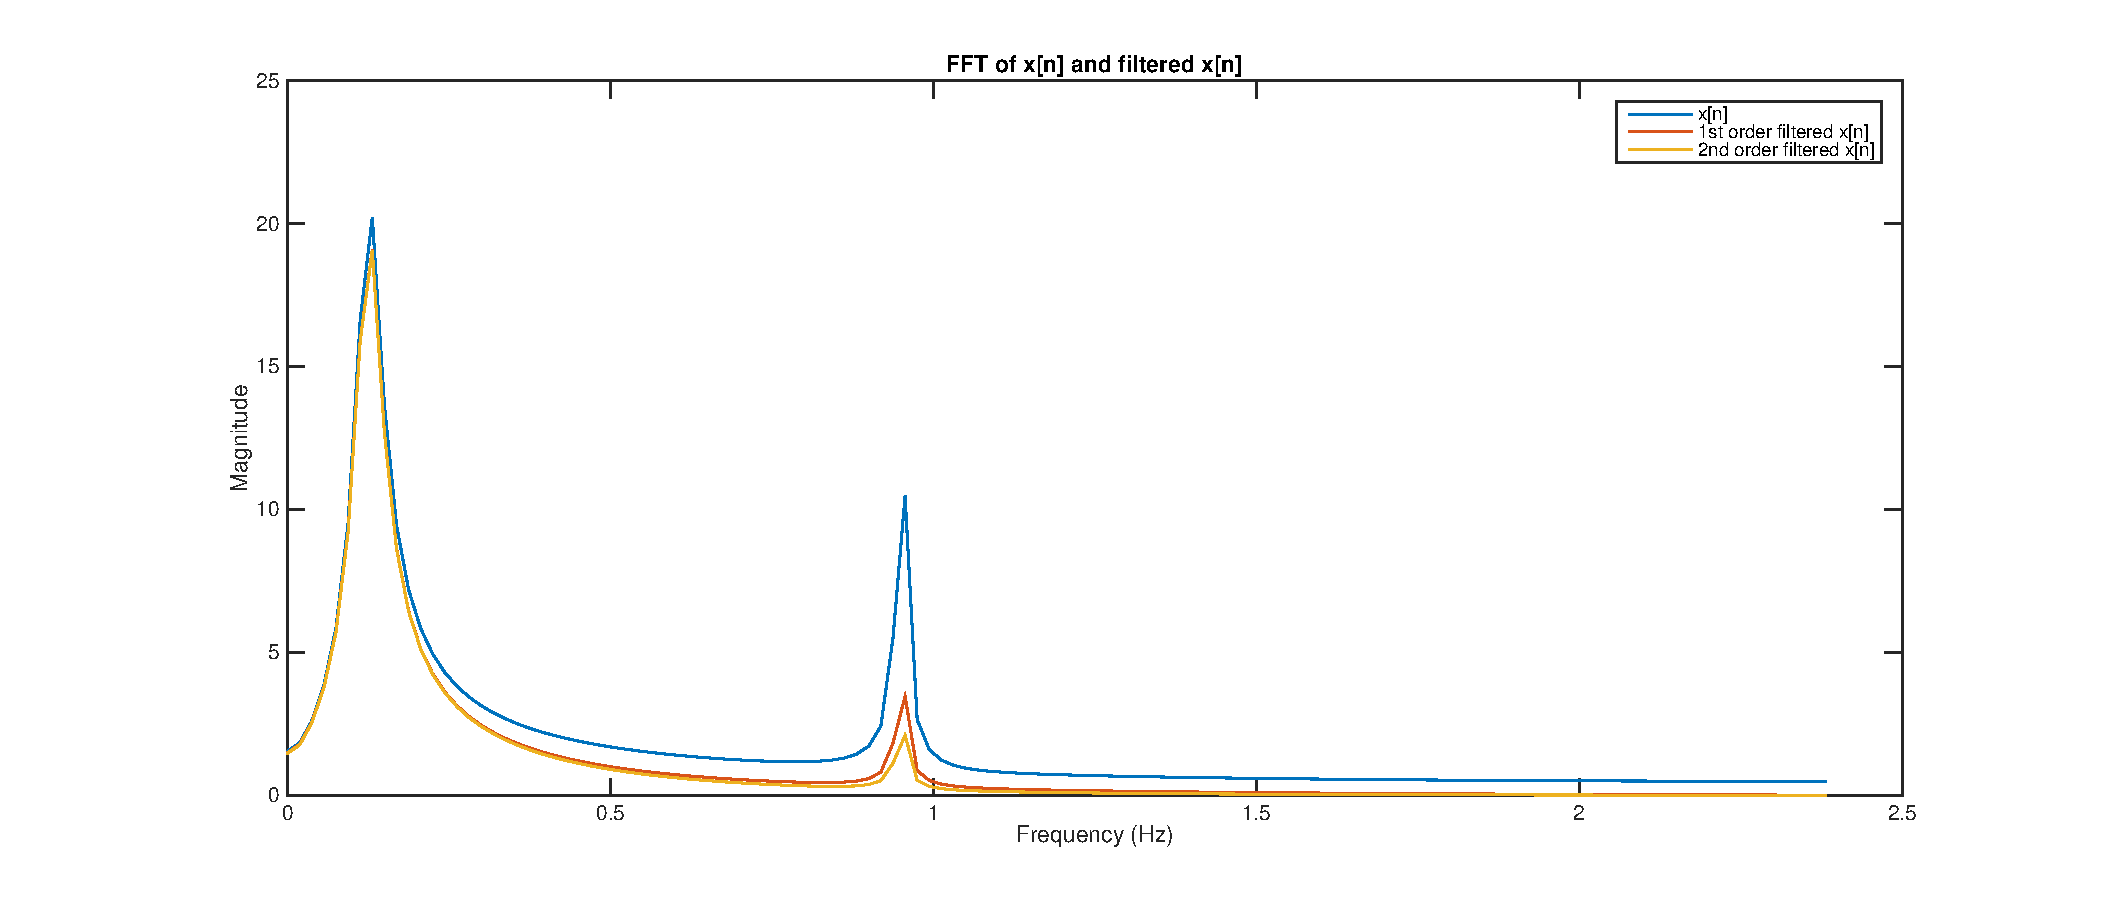
\includegraphics[width=6in]{Q2e-frequency.eps}
\caption{$x[n]$ and filtered $x[n]$ in frequency domain (MATLAB)}
\label{Q2e-frequency}
\end{figure}

\begin{figure}[H]
\centering
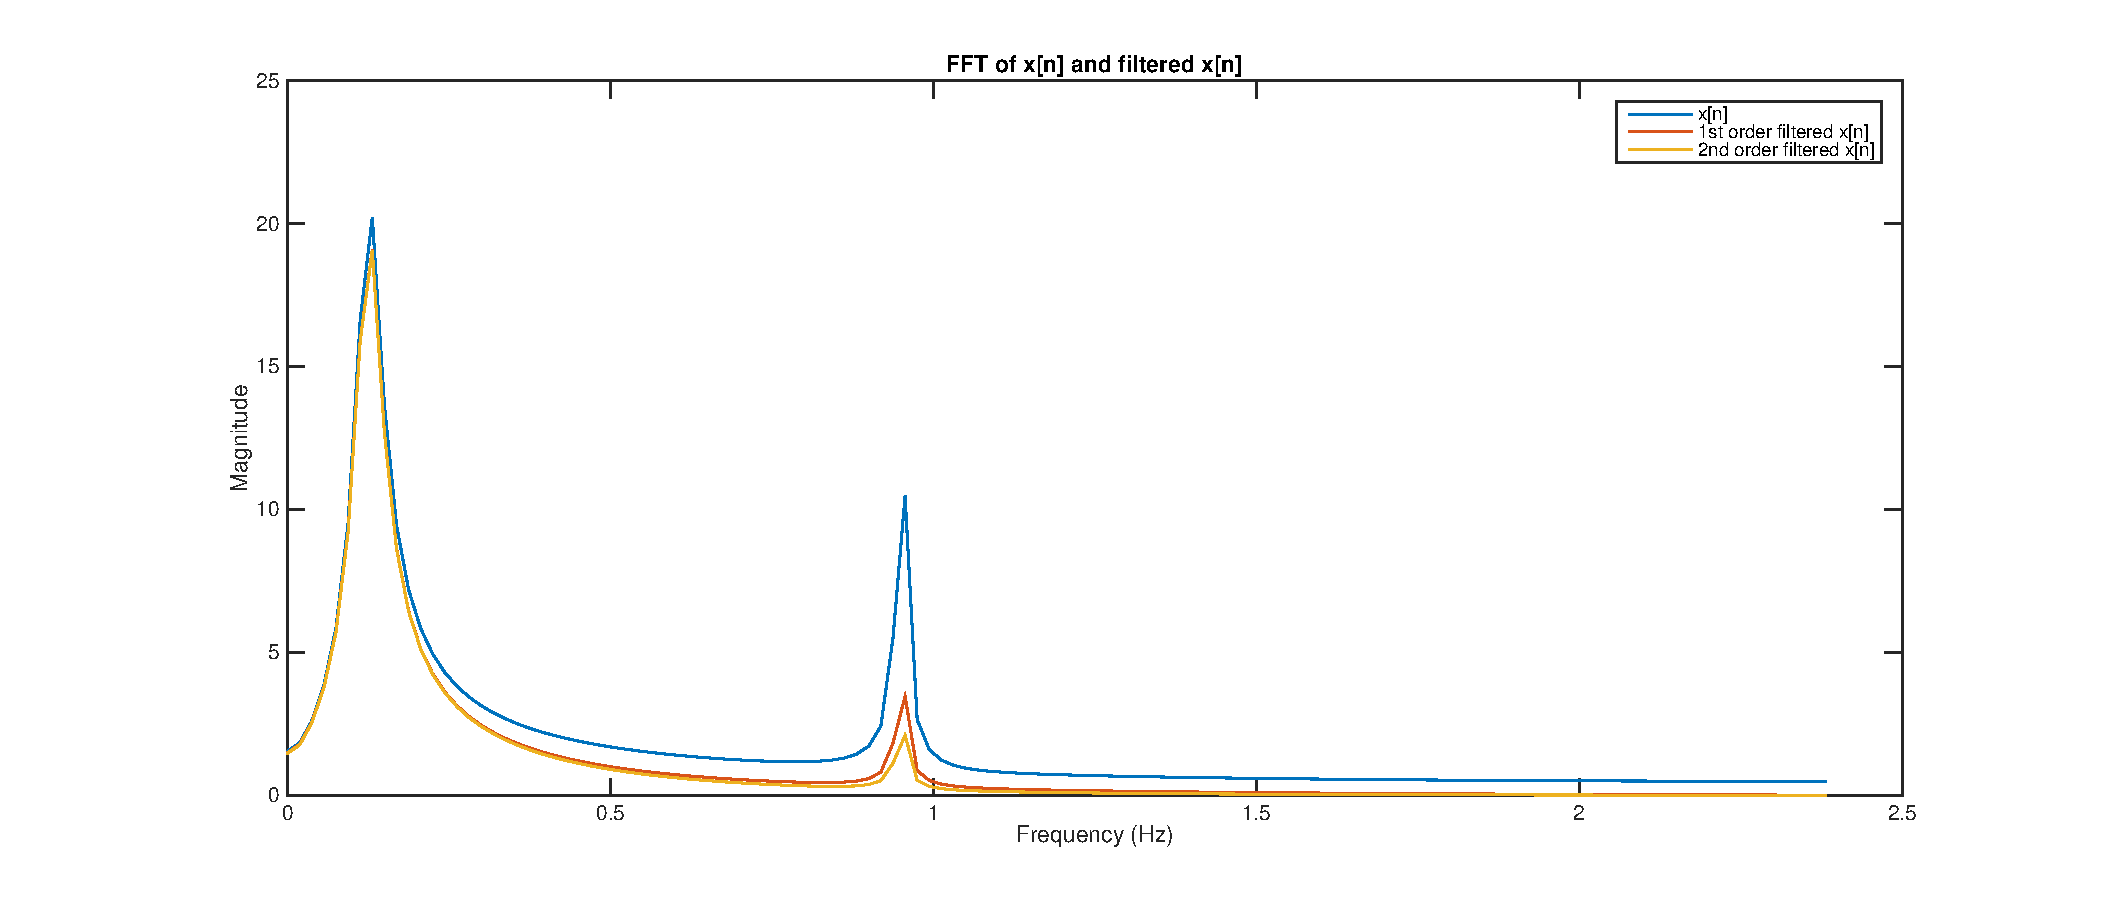
\includegraphics[width=6.6in]{Q2e-frequency}
\caption{$x[n]$ and filtered $x[n]$ in frequency domain (CCES)}
\label{Q2e-frequency-CCES}
\end{figure}

\problemAnswer{
\vspace{5pt}
Figure \ref{Q2e-frequency} and Figure \ref{Q2e-frequency-CCES} show analogous results. Looking at the frequency around $0.95\text{Hz}$, the magnitudes are 10.5, 3.5 and 2 respectively. Apparently,the second order filter successfully reduces the original signal down to about 20\% at frequency around $0.95\text{Hz}$. Looking at frequency around $0.125\text{Hz}$, the magnitudes are 20.1, 19.1 and 19.1 respectively. That is, the outputs from both filters achieve 95\% magnitude value around $0.125\text{Hz}$.\\

In conclusion, we eventually remove the component produced by $x_2[n]$ and keep the component induced by $x_1[n]$. 
}

%--------------------------------------------

\subsubsection*{f)}

\begin{figure}[H]
\centering
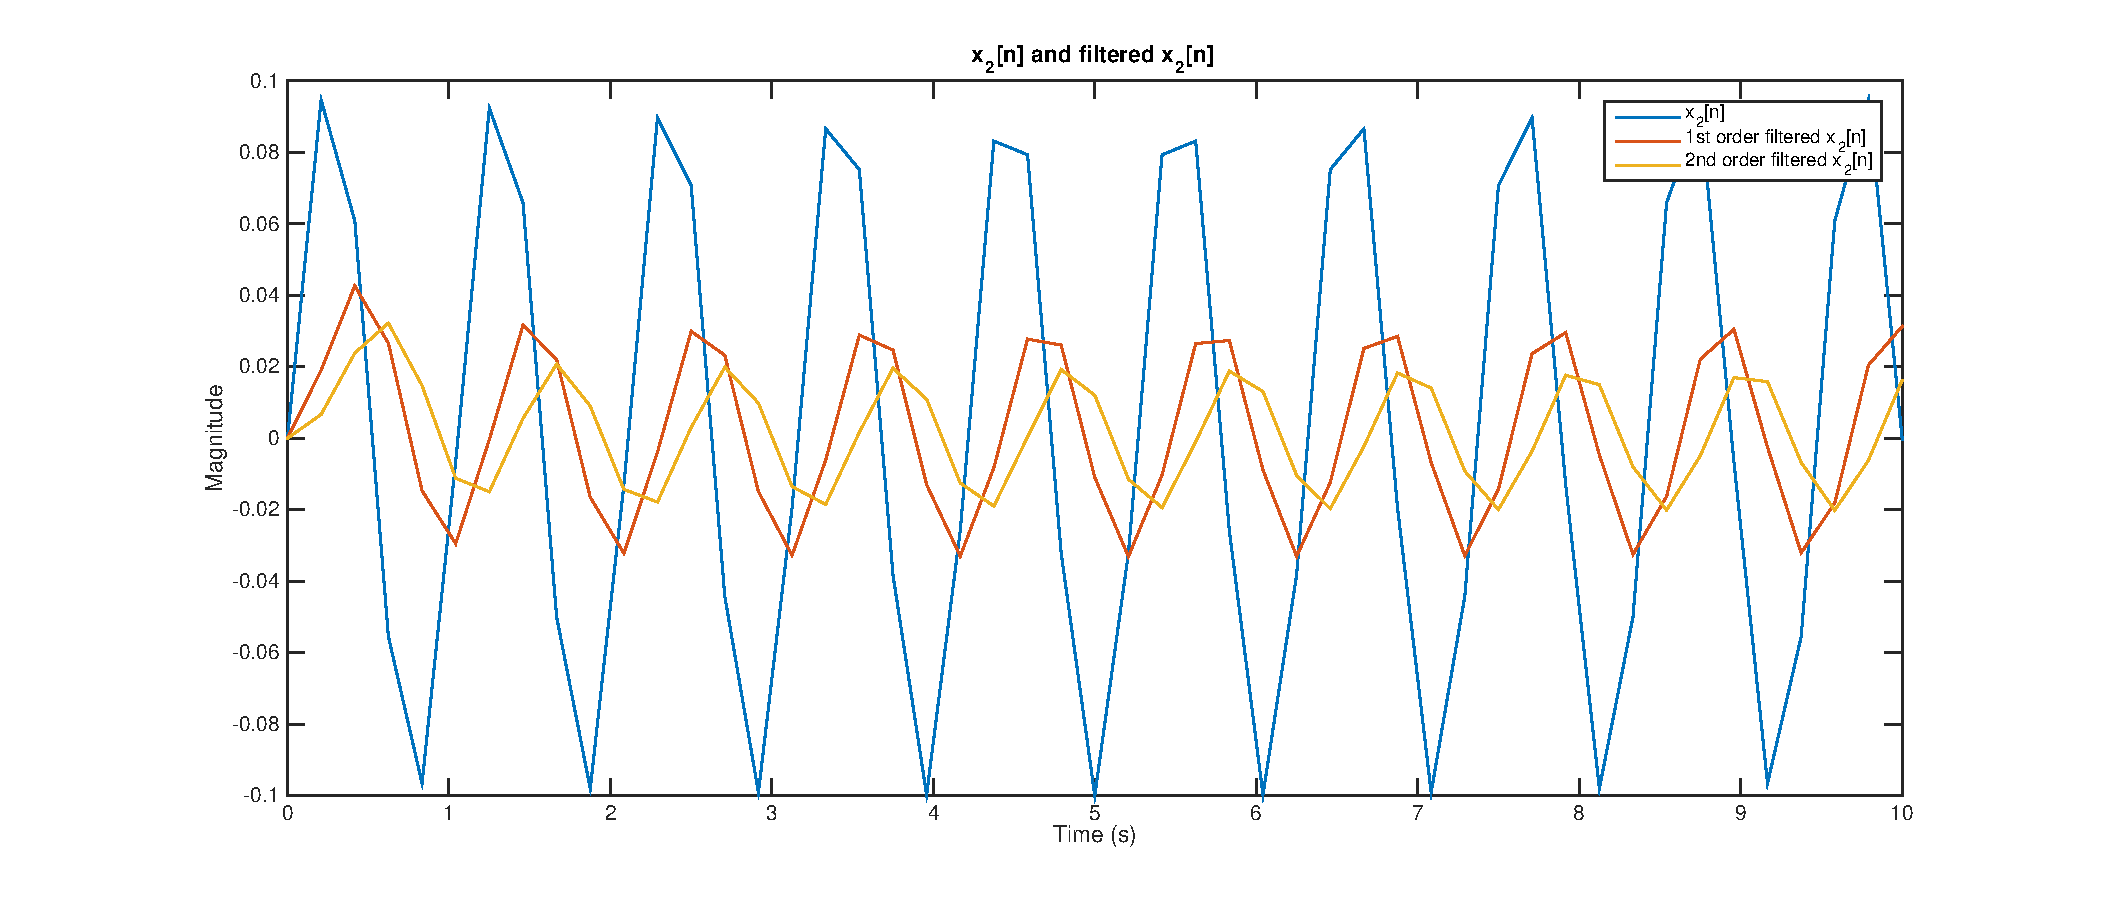
\includegraphics[width=6in]{Q2f.eps}
\caption{$x_2[n]$ and filtered $x_2[n]$ in time domain (MATLAB)}
\label{Q2f}
\end{figure}

\begin{figure}[H]
\centering
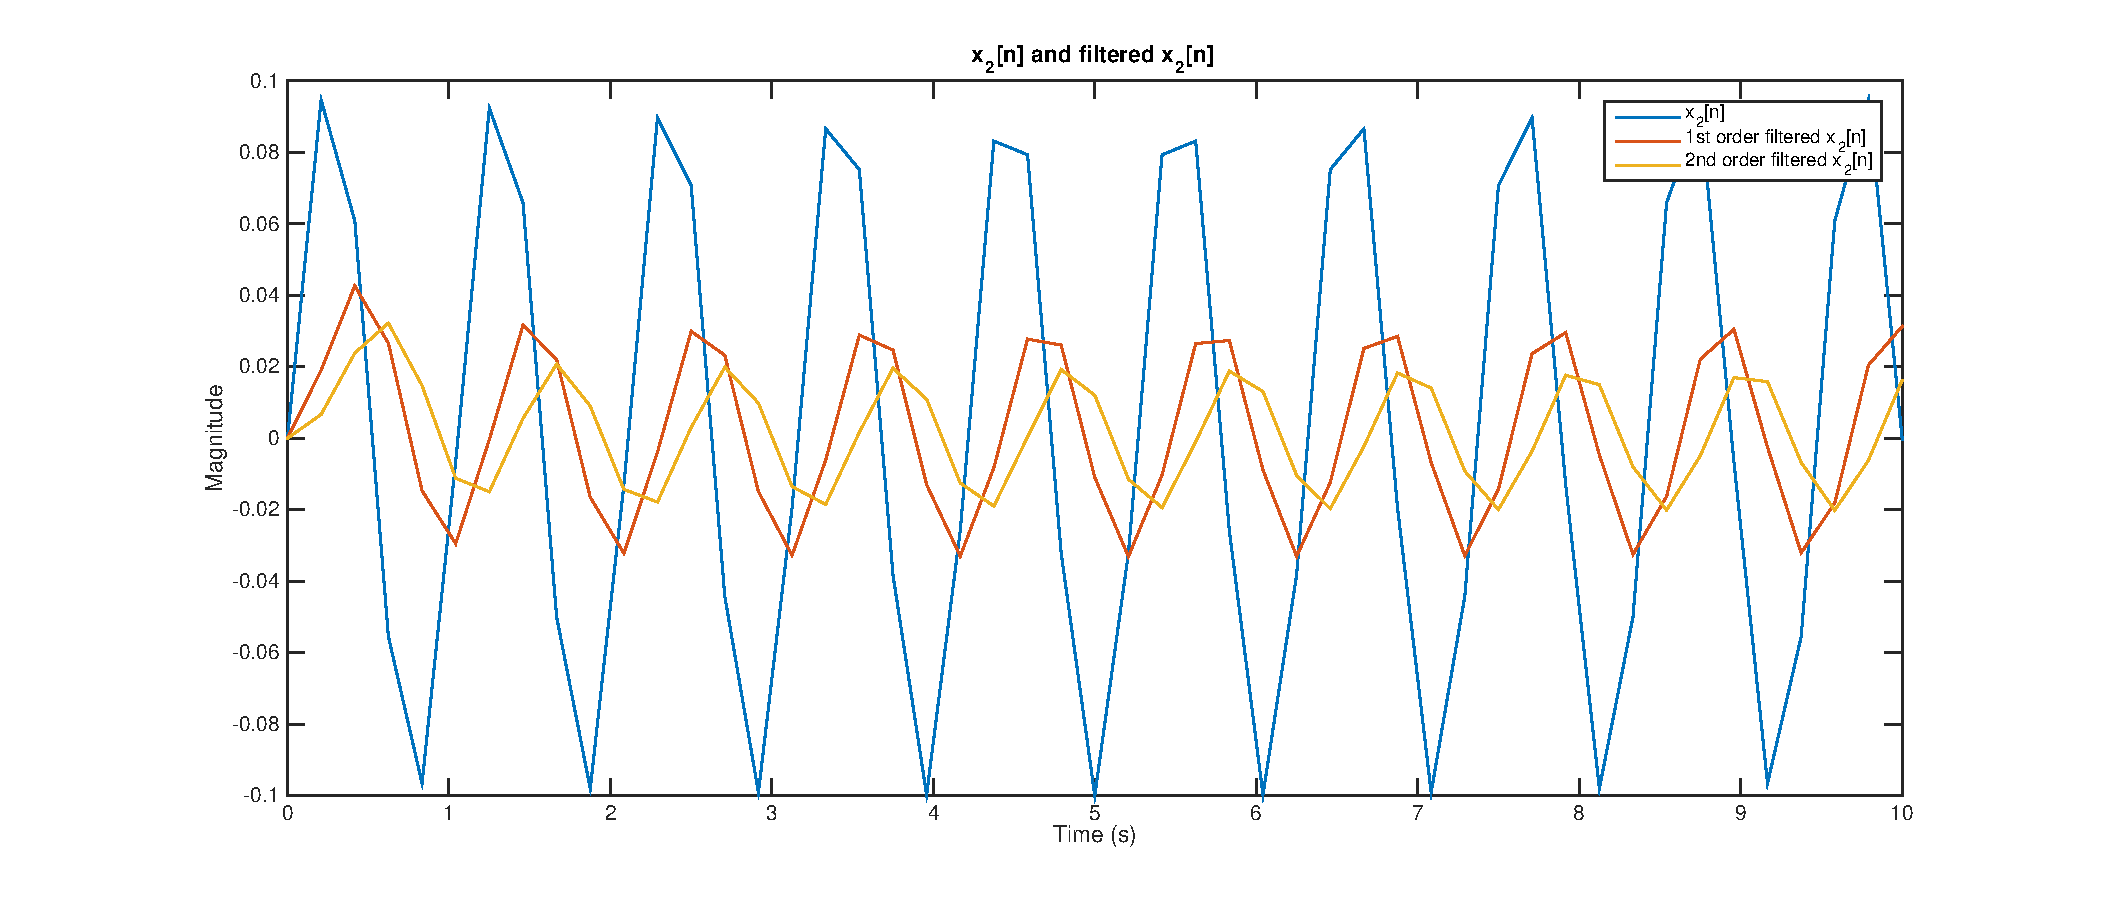
\includegraphics[width=6.6in]{Q2f}
\caption{$x_2[n]$ and filtered $x_2[n]$ in time domain (CCES)}
\label{Q2f-CCES}
\end{figure}

\problemAnswer{
\vspace{5pt}
From Figure \ref{Q2f} and Figure \ref{Q2f-CCES}, we can verify the gain by measuring the peak-to-peak value of each output.The original signal $x_2[n]$ has a peak-to-peak value 0.19 while the output of a second-order filter has 0.04 peak to peak value (21\% of 0.19) roughly. So the gain meets the requirement.\\

Second-order filter has better performance on gain attenuation, but at the expense of inducing larger phase shift. Time delay is more dramatic in second-order filter than the first-order filter.
}

%--------------------------------------------

\subsubsection*{g)}

\begin{figure}[H]
\begin{minipage}[t]{0.5\linewidth}
\centering
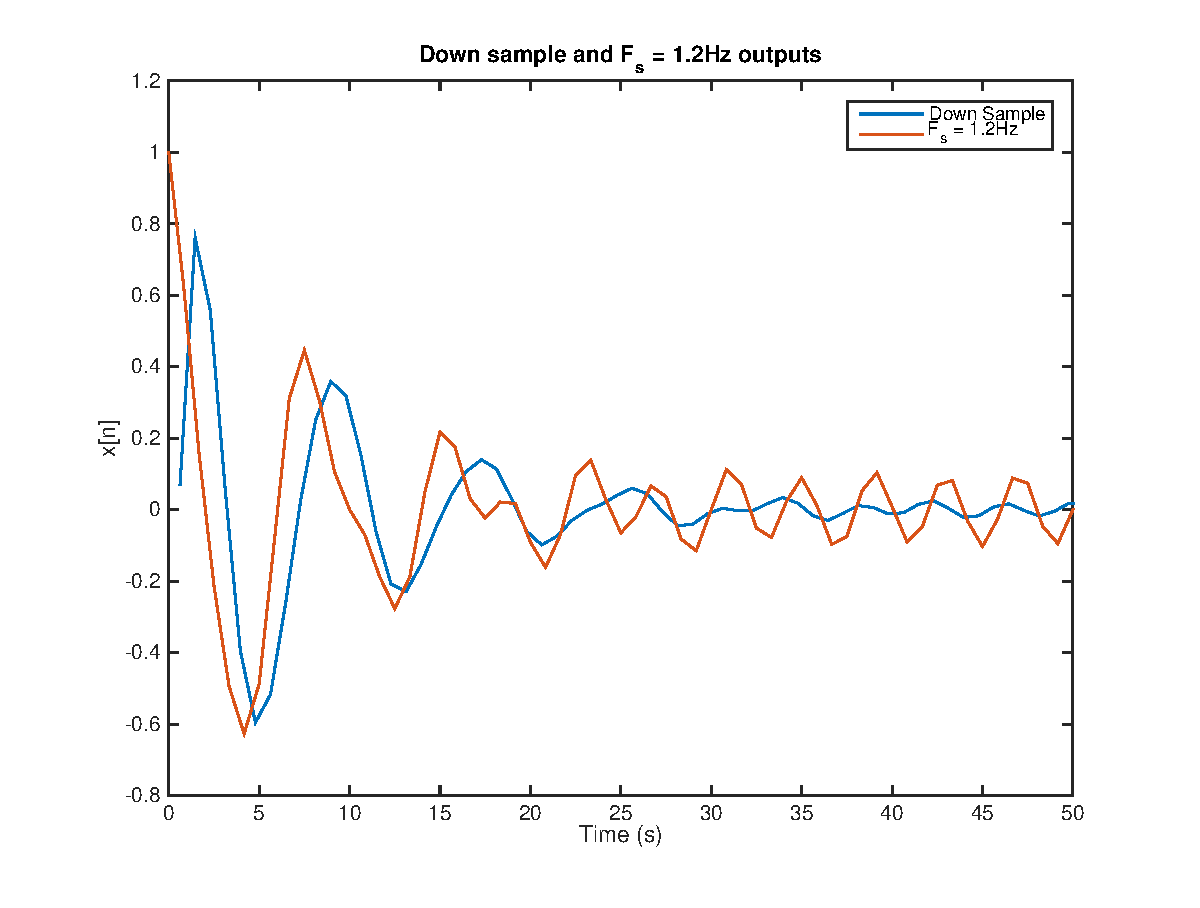
\includegraphics[width=3.3in]{Q2g-time.eps}
\caption{Down sample in time domain}
\label{Q2g-time}
\end{minipage}
\begin{minipage}[t]{0.5\linewidth}
\centering
\includegraphics[width=3.3in]{Q2g-frequency.eps}
\caption{Down sample in frequency domain}
\label{Q2g-frequency}
\end{minipage}
\end{figure}

\begin{figure}[H]
\centering
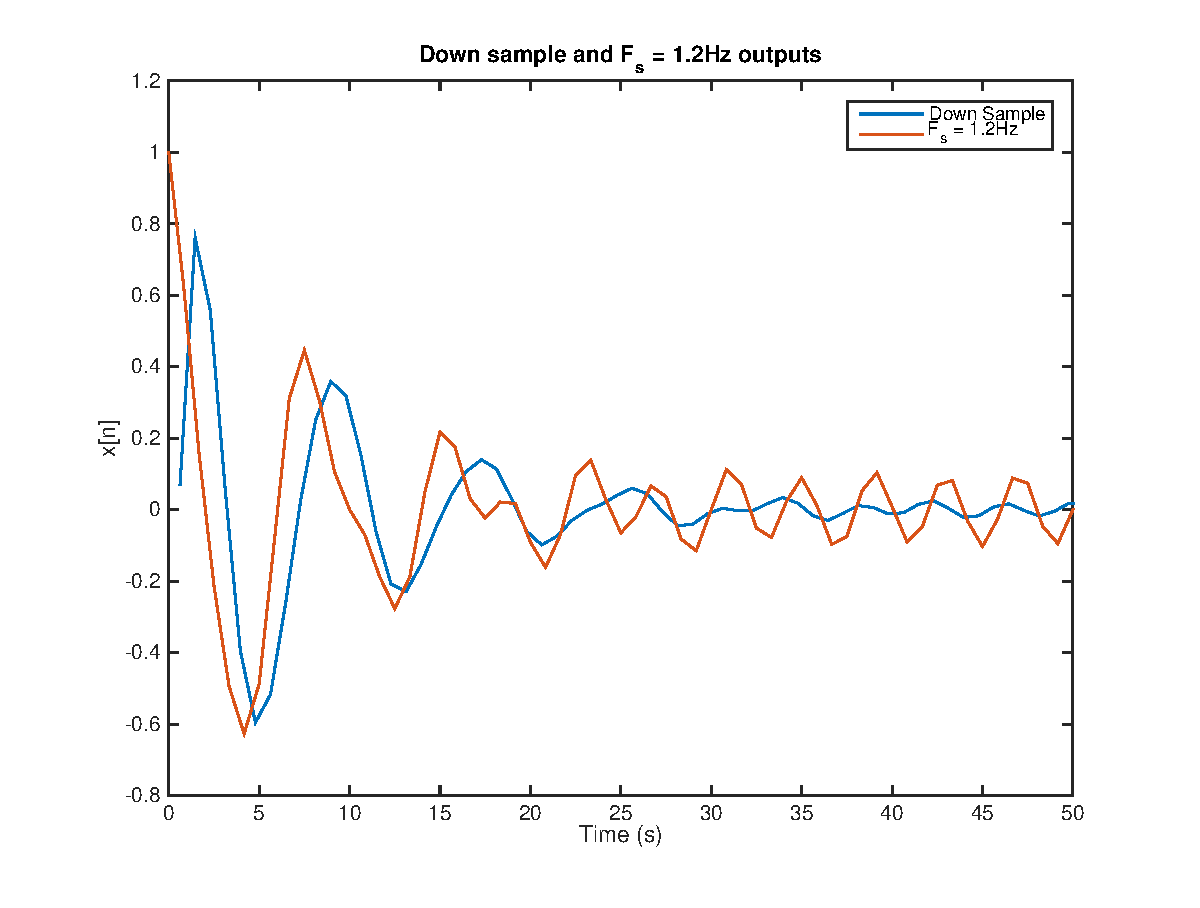
\includegraphics[width=6.6in]{Q2g-time}
\caption{Down sample in time domain (CCES)}
\label{Q2g-time-CCES}
\end{figure}

\begin{figure}[H]
\centering
\includegraphics[width=6.6in]{Q2g-frequency}
\caption{Down sample in frequency domain (CCES)}
\label{Q2g-frequency-CCES}
\end{figure}

\problemAnswer{
\vspace{5pt}
Based on our observation, in time domain, after down sampling $y[n]$, the peak-to-peak value of $y_{ds}[n]$ shrinks significantly which means we have removed the high frequency component in $y[n]$.\\

In frequency domain, seeing from Figure \ref{Q2g-frequency} and \ref{Q2g-frequency-CCES} , after down sampling, the folded peak around $0.248\text{Hz}$ disappears. Sampling frequency 4.8Hz is faster than twice the highest frequency of interest ($2 \times 1.9 \pi$ rad/s). The original signal is scarcely distorted after sampling. The second-order filter works as a digital anti-aliasing filter, high frequency components (e.g. at 0.95Hz) are attenuated effectively. After down sampling, de facto sampling frequency becomes 1.2Hz. 1.2Hz is still higher than twice of $0.25 \pi$ rad/s, hence no distortion occurs.
}

\end{homeworkSection}
\end{homeworkProblem}


%----------------------------------------------------------------------------------------
%	Appendix
%----------------------------------------------------------------------------------------

\newpage
\begin{homeworkProblem}{Appendix}

\begin{homeworkSection}{SPWS1.c}
\lstinputlisting[language=c]{SPWS1.c}
\end{homeworkSection}

\newpage
\begin{homeworkSection}{A a)}
\lstinputlisting{Q1a.m}
\end{homeworkSection}

\begin{homeworkSection}{A c)}
\lstinputlisting{Q1c.m}
\end{homeworkSection}

\begin{homeworkSection}{A d)}
\lstinputlisting{Q1d.m}
\end{homeworkSection}

\newpage
\begin{homeworkSection}{B.4 c) time domain}
\lstinputlisting{Q2c_time.m}
\end{homeworkSection}

\begin{homeworkSection}{B.4 c) frequency domain}
\lstinputlisting{Q2c_FFT.m}
\end{homeworkSection}

\begin{homeworkSection}{B.4 d) $\omega_{max}$ obtained from DTFT}
\lstinputlisting{Q2d_DTFT.m}
\end{homeworkSection}

\begin{homeworkSection}{B.4 d) $\omega_{max}$ obtained from FFT}
\lstinputlisting{Q2d_FFT.m}
\end{homeworkSection}

\begin{homeworkSection}{B.4 e) \& f) \& g)}
\lstinputlisting{Q2e_f_g.m}
\end{homeworkSection}

\end{homeworkProblem}

%----------------------------------------------------------------------------------------

\end{document}
